\documentclass[11pt, oneside]{article} 
\usepackage{amsmath, amsthm, amssymb, calrsfs, wasysym, verbatim, bbm, color, graphics, graphicx, geometry}
\usepackage[most]{tcolorbox}
\usepackage{xcolor}
\usepackage{framed}
\usepackage{caption}
\usepackage{subcaption}
%\colorlet{shadecolor}{blue!15}
\graphicspath{ {./figs} }

\geometry{tmargin=.75in, bmargin=.75in, lmargin=.75in, rmargin = .75in}  

\newcommand{\R}{\mathbb{R}}
\newcommand{\C}{\mathbb{C}}
\newcommand{\Z}{\mathbb{Z}}
\newcommand{\N}{\mathbb{N}}
\newcommand{\Q}{\mathbb{Q}}
\newcommand{\Cdot}{\boldsymbol{\cdot}}

%\newtheorem{thm}{Theorem}
%\newtheorem{defn}{Definition}
%\newtheorem{conv}{Convention}
%\newtheorem{rem}{Remark}
%\newtheorem{lem}{Lemma}
%\newtheorem{cor}{Corollary}
%\newtheorem{exa}{Ejemplo}

\newtcbtheorem[auto counter]{eje}%
  {Ejemplo}{fonttitle=\bfseries\upshape, fontupper=\slshape,
     arc=0mm, colback=blue!5!white,colframe=blue!75!black}{Ejemplo}

\newtcbtheorem[auto counter]{alg}%
  {Algoritmo}{fonttitle=\bfseries\upshape, fontupper=\slshape,
     arc=0mm, colback=red!5!white,colframe=red!75!black}{Algoritmo}

\title{Estructuras Hidr\'aulicas [2015961] \\ \textbf{Tema \# 2: Flujo uniforme}}
\author{\textbf{Luis Alejandro Morales, Ph.D}\\ \vspace{0.4cm} Profesor Asistente \\ Universidad Nacional de Colombia-Bogot\'a\\Facultad de Ingenier\'ia \\ Departamento de Ingenieria Civil y Agr\'icola}
%\date{Periodo 2022-II}
\date{}

\begin{document}

\maketitle
\tableofcontents

%\vspace{.25in}

%%%%%%%%
\section{Introducci\'on} % From Chau 
En flujo a superficie libre actuan basicamente dos fuerzas: \emph{fuerzas gravitacionales} cuya componente en direcci\'on del flujo en un canal de pendiente positiva acelera el flujo hacia abajo, y las \emph{fuerzas de fricci\'on} debido a la rugosidad del canal que tratan de frenar el flujo. Note que en un canal con pendiente negativa, el flujo trata de desacerelarse. En un canal con pendiente positiva, si las fuerzas de fricci\'on son mayores que las fuezas gravitacionales, el flujo se sesacelera produciendo una elevacion de la lamina de agua, lo cual se da gracias al principio de \emph{coservacion de la masa}. En el caso contrario la profundidad de la lamina de agua disminuye y la velocidad aumenta. En canales prismaticos largos, es posible que las dos fuerzas se igualen en alguna secci\'on del canal haciendo que ni la profundidad ni la velocidad cambien a partir de este punto aguas abajo (ver figura~\ref{fig1}). Por lo tanto, en un flujo en el cual la profundidad no cambia se le denomina \emph{flujo uniforme} y a la profundidad del flujo \emph{profundidad normal}.

% Chau fig 4.1
\begin{figure}[h]
\centering
%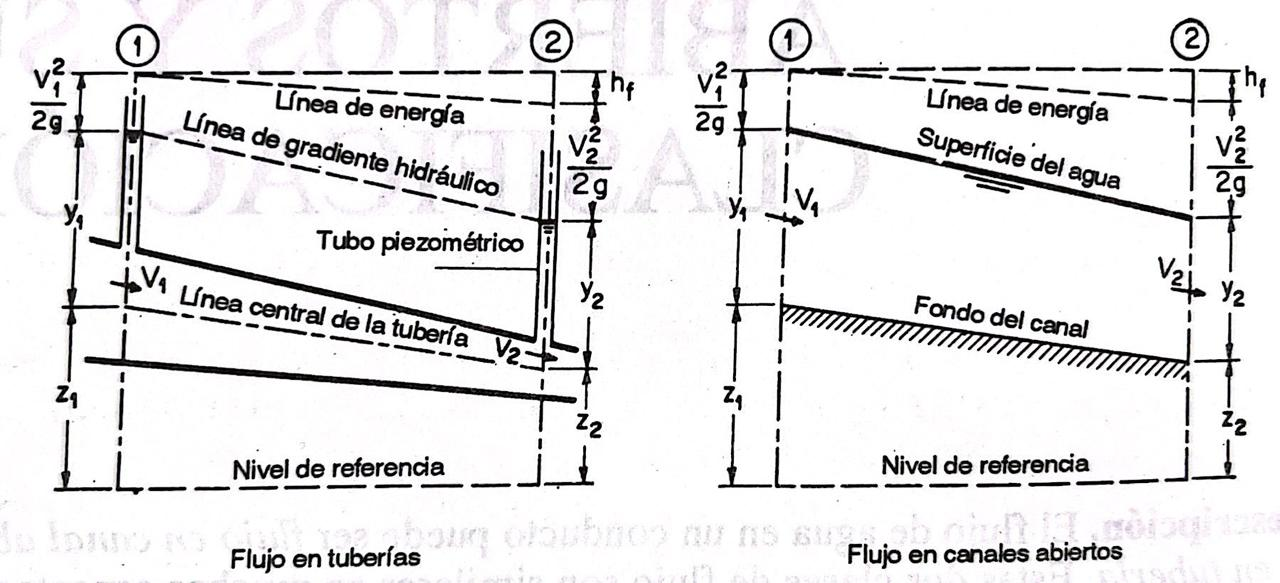
\includegraphics[width=8cm]{fig1.jpeg}
\caption{Flujo no uniforme y uniforme en canales (tomado de \cite{Chau}).}
\label{fig1}
\end{figure}


\section{Resistencia al flujo} % From Chau 
En un canal es notorio que la velocidad aumenta desde las orillas y hacia el centro. Lo mismo ocurre al analizar un perfil de velociades en un canal donde las velocidades aumentan desde el fondo hacia la superficie. Esto se presenta debido a la resistencia al movimiento que ofrece el material del fondo y las orillas del canal que suele ser mas pesado que el fluido en movimiento y que el aire que esta en la superficie. A pesar que en la realidad los esfuerzos cortantes no son uniformes sobre el perimetro mojado del canal y que existen corrientes secundarias en una secci\'on transversal, para efectos practicos consideraremos flujo 1D lo que implica velocidades y esfuerzos uniformes en la secci\'on. 

\subsection{Ecuaciones para la resistencia al flujo}
En esta secci\'on se presentan algunas ecuaciones que relacionan la resistencia al flujo con otras variables del flujo para, inicialmente, flujo no uniforme, las cuales al simplifircarse se usan en flujo uniforme. 

\subsubsection{Ecuaci\'on de Chezy}
Consideremos un flujo permanente en un canal prismatico y de pendiendiente baja. Si analizamos un volumen de control dentro del flujo entre dos secciones 1 y 2, la primera a una distancia $x$ y la otra a una distancia $x + \Delta x$ a lo largo del canal, en donde la profundidad y la velociadad en 1 es $y$ y $V$, respectivamente, aguas abajo en 2 tenemos que la profundidad es $y + \frac{dy}{dx} \Delta x$ y $V + + \frac{dV}{dx} \Delta x$ (ver figura~\ref{fig2}) Analizando las fuerzas actuantes sobre el volumen de control se tenemos: una fuerza de presi\'on en la seccion 1, $F_1$; fuerzas de presi\'on en la secci\'on de salida 2, $F_2$ y $F_3$; componente del peso del fluido en la direcci\'on del flujo, $W_x$; y la fuerza de fricci\'on en en el fondo y paredes del canal que se opone al movimiento, $F_f$. 

% Chau fig 4.2
\begin{figure}[h]
\centering
%\includegraphics[width=8cm]{fig2.jpeg}
\caption{Fuerzas actuantes en un volumen de contro de un flujo en un canal (tomado de \cite{Chau}).}
\label{fig2}
\end{figure}

La  fuerza de presi\'on en la secci\'on 1 se calculan como $F_1 = \gamma A \bar{z}$, donde $A$ es el area mojada de la secci\'on transversal 1 y $\bar{z}$ es la profundidad del centroide de la secci\'on. La componente del peso en la direcci\'on del flujo se calcula como $W_x = \gamma A \Delta x \sin \theta$, donde $\theta$ es el \'angulo de pendiente del canal. Note que como la pendiente del canal es baja, $\sin \theta \simeq \tan \theta \simeq  -dz/dx$, por lo tanto $W_x = -\gamma A \Delta x \frac{dz}{dx}$. En las secci\'on 2, aguas abajo, actual dos fuerzas de presi\'on: la fuerza debido a la profundidad ($F_2$) y la fuerza debido a la sobre-elevaci\'on en la distancia $\Delta x$ ($F_3$). De acuerdo con esto, $F_2 = \gamma A \bar{z}$ y $F_3 = \gamma A \frac{dy}{dx} \Delta x$. Como los esfuerzos cortantes ($\tau_o$) sobre las paredes y el fondo del canal son uniformes, la fuerza de fricci\'on se puede calcular como $F_f = \tau_o P \Delta x$, donde $P$ es el perimetro mojado de la secci\'on. 

Haciendo sumatoria de las fuerzas actuantes sobre el volumen de control en la direcci\'on del flujo de la figura~\ref{fig2}, la fuerza resultante ($F_r$) es:
\begin{equation}
 F_r = \sum F = F_1 - F_2 - F_3 + W_x - F_f 
\label{eq1}
\end{equation}

Sustituyendo las expresiones para cada fuerza en la ecuaci\'on~\ref{eq1}, tenemos:
\begin{equation}
 F_r = -\gamma A \Delta x \left( \frac{dy}{dx} + \frac{dz}{dx} + \frac{P \tau_o}{\gamma A} \right)
\label{eq2}
\end{equation}

Aplicando la ley de conservacion de la cantidad de movimiento para el volumen de control de la figura~\ref{fig2}, la cual establece que la tasa de cambio de la cantidad de movimiento es igual a la fuerza resultante e igual a $F_r = \rho AV (V_2 - V_1) = \rho AV \left( \left( V + \frac{dV}{dx}\Delta x \right) - V \right) = \rho A V \frac{dV}{dx} \Delta x$. Igualando a la ecuaci\'on~\ref{eq2} y dividiendo por $\gamma A \Delta x$:
\begin{equation}
\frac{V}{g}\frac{dV}{dx} = -\left( \frac{dy}{dx} + \frac{dz}{dx} + \frac{P \tau_o}{\gamma A} \right)
\label{eq3}
\end{equation}

Despejando $\tau_o$ de esta ecuaci\'on:
\begin{equation}
\tau_o = -\gamma R \left( \frac{V}{g}\frac{dV}{dx} + \frac{dy}{dx} + \frac{dz}{dx} \right)
\label{eq4}
\end{equation}

donde $R=A/P$ es el radio hidr\'aulico. Simplificando la ecuacion anterior:

\begin{equation}
\tau_o = -\gamma R \frac{d}{dx} \left( z + y + \frac{V^2}{2g} \right) = -\gamma R \frac{dH}{dx} = \gamma R S_f
\label{eq5}
\end{equation}

donde $H$ es la energ\'ia total en una secci\'on del flujo y $S_f = -\frac{dH}{dx}$ es la p\'erdida de energ\'ia en la direcci\'on del flujo o pendiente de la l\'inea de energia. Para flujo uniforme, los terminos  $\frac{dV}{dx}$ y  $\frac{dy}{dx}$ de la ecuaci\'on~\ref{eq5} son iguales a cero y la $S_f = S_o = -\frac{dz}{dx}$. Para flujo uniforme, la ecuaci\'on~\ref{eq5} queda:
\begin{equation}
\tau_o =  \gamma R S_o
\label{eq6}
\end{equation}

Por otra parte, con base en \emph{analisis dimensional}, se tiene que:
\begin{equation}
\tau_o = \kappa \rho V^2
\label{eq7}
\end{equation}

donde $\kappa$ es un coeficiente adimensional que depende del n\'umero de Reynolds ($Re$) y de la rugosidad de canal. Igualando las ecuaciones~\ref{eq5} y ~\ref{eq7} y despejando para $V$, tenemos:
\begin{equation}
V = \sqrt{\frac{g R S_f}{\kappa}}
\label{eq8}
\end{equation}

La ecuaci\'on~\ref{eq8} puede ser escrita como:
\begin{equation}
\color{red}\boxed{\color{black} V = C\sqrt{R S_f}}
\label{eq9}
\end{equation}

donde $C = \sqrt{\frac{g}{\kappa}}$ es el  \emph{coeficiente de Chezy}. Note que la ecuaci\'on~\ref{eq9} es para flujo permanente y no uniforme. Para el caso del flujo permanente y uniforme, igualando las ecuaciones~\ref{eq6} y ~\ref{eq7}, se tiene:
\begin{equation}
\color{red}\boxed{\color{black} V = C\sqrt{R S_o}}
\label{eq10}
\end{equation}

Note que en flujo uniforme, la pediente de la linea de energia, la pendiente de la linea de gradiente hidraulico y la pendiente del canal son iguales.

Por otro lado, $C$ tiene unidades de $\sqrt{L}/T$ y depende de $R_e$ y de la rugosidad del canal. La \emph{ecuaci\'on de Darcy-Weisbach} para tuber\'ias:
\begin{equation}
h_f = f\frac{L}{D}\frac{V^2}{2g}
\label{eq11}
\end{equation}

donde $f$ es un factor de fricci\'on adimensional que depende de $R_e$ y de la rugosidad de la tuber\'ia, $D$ es el diametro de la tuber\'ia y $L$ es la longitud de la tuber\'ia, se puede simplificar:
\begin{equation}
V = \sqrt{\frac{2g D S}{f}}
\label{eq12}
\end{equation}

donde $S = \frac{h_f}{L}$. La ecuaci\'on~\ref{eq9}, se convierte en, donde $R=D/4$:
\begin{equation}
V = C\sqrt{\frac{D S}{4}}
\label{eq13}
\end{equation}

Igualando las ecuaciones~\ref{eq12} y ~\ref{eq13}, se tiene que:
\begin{equation}
C = \sqrt{\frac{8g}{f}}
\label{eq13}
\end{equation}

El \emph{diagrama de Moody} se puede expresar en funci\'on de $C$ y del $R_e$ (ver figura~\ref{fig3}). Este diagrama esta divido en tres regiones que reflejan en tipo de fljo: hidraulicamente lisa, transici\'on y totalmente rugosa. Un flujo en la region hidraulicamente lisa es un flujo laminar que no necesarimente posee una rugosidad baja. En la medida en que $R_e$  aumenta, la subcapa laminar decrese y los efectos rugosos son importante entrando en la region de transici\'on. Sin embargo cuando la rugosidad no es cubierta por la subcapa viscosa y existen perdidas de energia, el flujo es clasificado como completamente rugoso. El flujo se puede clasificar dependiendo  al numero adimensional $R_s = \frac{k V^* }{\nu}$, donde $\nu$ es la viscosidad cinem\'atica del fluido y $k$ es una longitud caracteristica de la rugosidad de la superficie del canal. $V^*$ es la velocidad cortante expresada como $V^* = \sqrt{\frac{\tau_o}{\rho}}=\sqrt{gR S_f}$. Por lo tanto:

% Chau fig 4.3
\begin{figure}[h]
\centering
%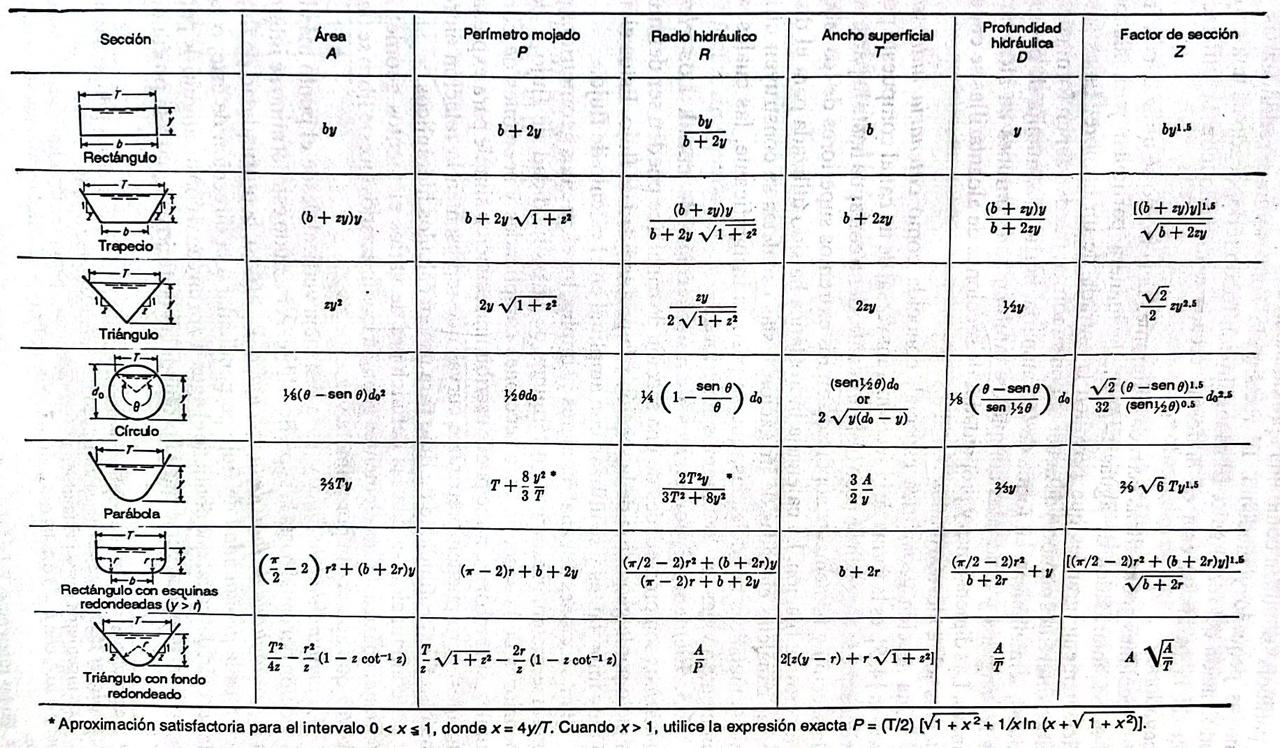
\includegraphics[width=8cm]{fig3.jpeg}
\caption{Diagrama de Moody modificado (tomado de \cite{Chau}).}
\label{fig3}
\end{figure}

\begin{itemize}
\item Si $R_s < 4$, \emph{flujo hidraulicamente liso}
\item Si $4 < R_s < 100$, \emph{flujo de transici\'on}
\item Si $R_s > 100$, \emph{flujo completamente rugoso} 
\end{itemize}
Existen expresiones experimentales para calcular $C$ para para el caso de canales relativamente pequeños de superficie lisa ya que estas expresiones fueron obtenidas con base en experimentos en tuber\'ias. 

\begin{itemize}
\item \textbf{Flujo liso}
\begin{equation}
C = \begin{cases}
28.6 R_e^{1/8} & \text{if $R_e < 10^5$;}\\
4\sqrt{2g}\log_{10} \left( \frac{R_e \sqrt{8g}}{2.51 C}\right) & \text{if $R_e > 10^5$;}
\end{cases}
\label{eq14}
\end{equation}

\item \textbf{Flujo rugoso}
\begin{equation}
C = -2\sqrt{8g}\log_{10} \left(\frac{k_s}{12R} + \frac{2.5}{R_e \sqrt{f}} \right)
\label{eq15}
\end{equation}
\end{itemize}

\subsubsection{Ecuaci\'on de Manning}
Desde la derivaci\'on de la ecuaci\'on de Chezy, muchos investigadores han tratado de derivar una expresi\'on para calcular $C$. Sin embargo, debido a que $C$ depende de muchas variables, encontrar una expresion para $C$ no ha sido facil. Con base en observaciones de campo, Gauckler y Hagen mostraron que $C \propto R^{1/6}$. El Irlandes R. Manning en 1891, encontro la siguiente ecuaci\'on a partir de la ecuaci\'on de Chezy:
\begin{equation}
\color{red}\boxed{\color{black} V = \frac{C_o }{n} R^{2/3} S_f^{1/2}}
\label{eq16}
\end{equation}

donde $n$ es el \emph{coeficiente de rugosidad de Manning} y tiene unidades de $L^{1/3} /T$; $C_o$ es un coeficiente de conversi\'on de unidades cuyo valor es $C_o = 1.0$ en \emph{sistema internacional de unidades (SI)} y $C_o = 1.49$ en \emph{sistema Ingl\'es de unidades (BG)}. $V$ est\'a dada en $m/s$ y $R$ en $m$ en SI, y $V$ esta dada en $ft/s$ y $R$ en $ft$ en BG.
 
Note que el valor de $n$ es el mismo en ambos sistemas. $n$ depende principalmente de la rugosidad del material del canal, de las irregularidades y de la profundidad de la lamina de agua, entre otros. La tabla~\ref{ta1} muestra los valores m\'as comunes para diferentes tipos de canal y se puede observar como $n$ aumenta en la medida en que el canal se hace m\'as rugoso; los canales naturales poseen los mayores valores de $n$ (ver figura~\ref{fig4}).   

\begin{table}[h!]
\centering
\begin{tabular}{l c}
 \hline
  Material & $n$ \\ [0.5ex]
 \hline\hline
 \emph{Metales} & \\
 Acero & 0.012 \\
 Hierro fundido & 0.013 \\
 Metal corrugado & 0.025 \\
 \emph{No metales} & \\
 Lucita & 0.009 \\
 Vidrio & 0.010 \\
 Cemento & 0.011 \\
 Concreto & 0.013 \\
 Madera & 0.012 \\
 Arcilla & 0.013 \\
 Ladrillo & 0.013 \\
 Hormigon lanzado & 0.019 \\
 Mamposteria & 0.025 \\
 Roca cortada & 0.035 \\
 \emph{Canales naturales} & \\
 Limpios y derechos & 0.030 \\
 Fondo con arena y gravilla & 0.040 \\
 Fondo con grava y roca & 0.050 \\
\hline
\end{tabular}
\caption{Coeficientes de rugosidad de Manning $n$ (tomado de \cite{VChow}).}
\label{ta1}
\end{table}

% Chau fig 4.4
\begin{figure}[h]
\centering
%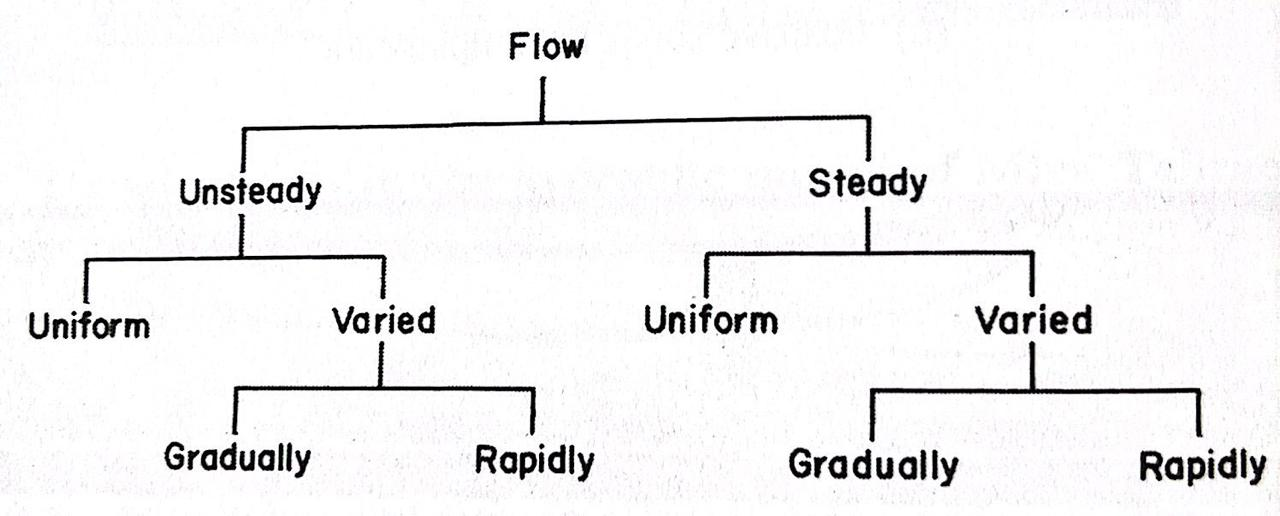
\includegraphics[width=8cm]{fig4.jpeg}
\caption{Valores de $n$ para canales naturales: a) Rio Columbia, Washington, $n=0.024$, b) Quebrada Salada, Nebraska, $n=0.030$, c) Rio Salado, Arizona, $n=0.032$ y d) Rio Bitteroot, Montana, $n=0.036$  (tomado de \cite{Chau}).}
\label{fig4}
\end{figure}

El coeficiente de Manning es dificil de estimar ya que depende de varias variables. Investigaciones han demostrado que $n$ aumenta en la medida en que la profundidad de la lamina de agua disminuye. En canales revestidos, es comun trabajar con un valor de $n$ constante. Sin embargo cuando la lamina de agua disminuye el valor de $n$ aumenta. Para canales revestidos con material granular y rocoso 
$$
n=C_m \left( 3.28 d_{50} \right)^{1/6} 
$$
donde $d_{50}$ es el diametro medio de la grava en $m$, $0.034 \leq C_m \leq 0.039$ para canales con fondo en gravilla. Otra ecuaci\'on  similar es:
$$
n = \frac{\left( R/0.3048 \right)^{1/6}}{8.6 + 19.97 \log \left( R/d_{50} \right)} 
$$
donde $R$ es el radio hidr\'aulico en $m$. Valores de $n$ para diferentes recubrimientos y diferentes rangos de profundidad se muestran en la figura~\ref{fig5}.

% Chau tab 4.2
\begin{figure}[h]
\centering
%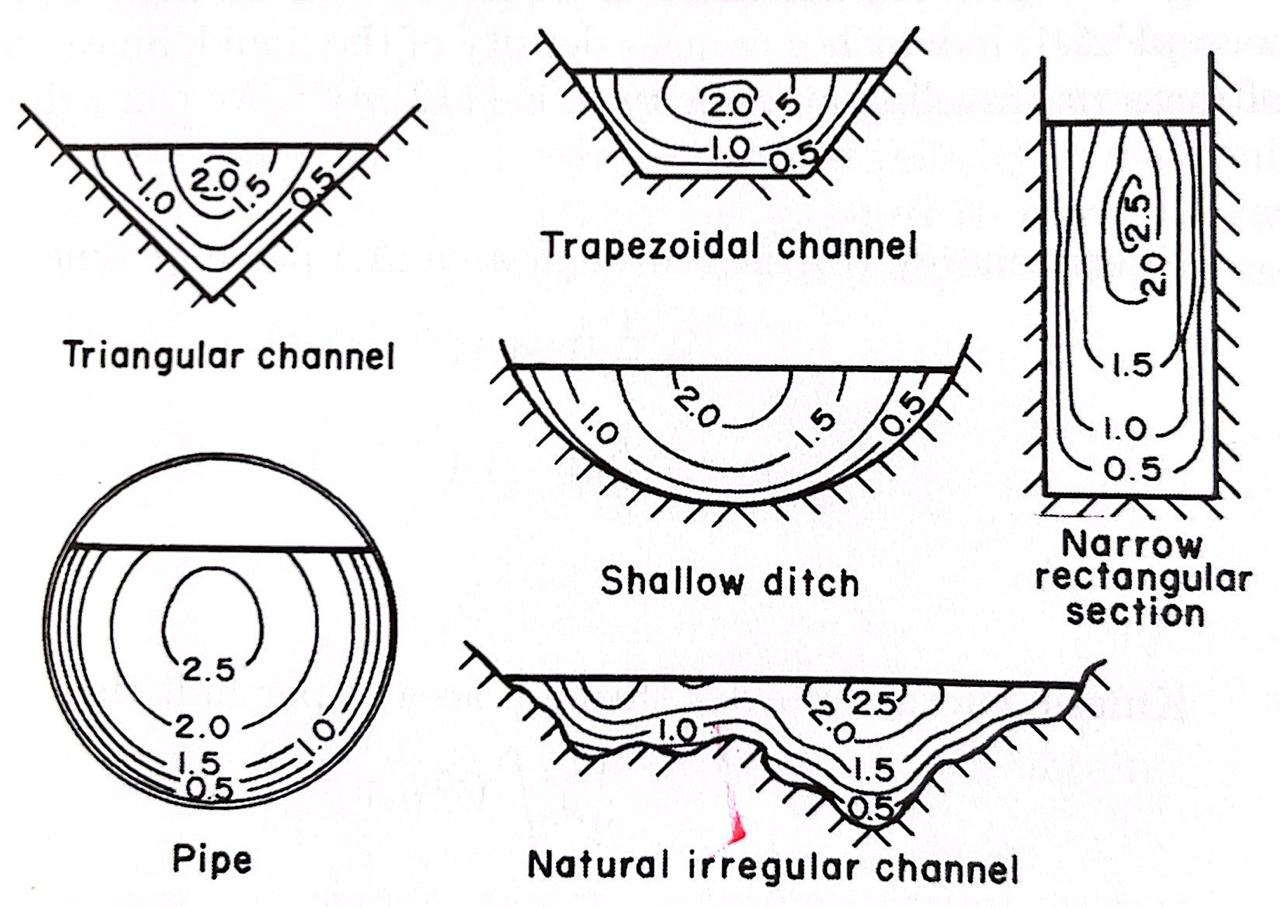
\includegraphics[width=8cm]{fig5.jpeg}
\caption{Valores de $n$ para diferentes recubrimientos y rangos de profundidades (tomado de \cite{Chau}).}
\label{fig5}
\end{figure}

Para canales revestidos con vegetaci\'on, un $n$ constante no es adecuado, teniendo que la cantidad de vegetaci\'on sumergida cambia con el nivel y de igual manera los esfuerzos cortantes. Para estos casos tenemos que:
$$
n=\frac{\left( R/0.3048 \right)^{1/6}}{C + 19.97 \log \left[ \left( R/0.3048 \right) \right]^{1.4} S_o^{0.4}}
$$
donde $R$ es el radio hidraulico en $m$, $S_o$ es la pendiente del fondo del canal y $C$ es un coeficiente adimensional que depende del tipo de vegetaci\'on. La figura~\ref{fig6} muestra valores de $C$ para diferentes tipos de vegetaci\'on. 

% Chau tab 4.3
\begin{figure}[h]
\centering
%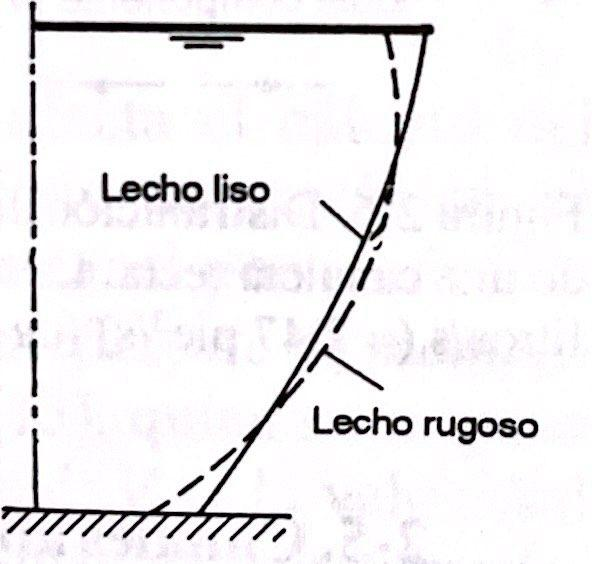
\includegraphics[width=8cm]{fig6.jpeg}
\caption{Valores de $C$ para diferentes tipos de recubrimiento con vegetaci\'on (tomado de \cite{Chau}).}
\label{fig6}
\end{figure}

\subsubsection{Otras ecuaciones de resistencia}
En Europa, la \emph{ecuaci\'on de Strickler} has sido ampliamente usada:
\begin{equation}
\color{red}\boxed{\color{black} V = k_s R^{2/3} S_f^{1/2}}
\label{eq18}
\end{equation}

donde $k_s$ es la \emph{constante de Strickler}, la cual en sistema internacional se calcula como $k_s = \frac{21.1}{k^{1/6}}$ donde $k$ es la rugosidad media del material en $mm$. Alguno valores de $k$ se muestran en la tabla~\ref{ta2}.

\begin{table}[h!]
\centering
\begin{tabular}{l c}
 \hline
  Material & $k$ (mm) \\ [0.5ex]
 \hline\hline
 Hierro fundido nuevo & 0.5-1.0 \\
 Hierro fundida usado & 1.0-1.5 \\
 Acabado en cemento & 0.3-0.8 \\
 Acabado rugoso en cemento & 1.0-2.0 \\
 Madera rugosa & 1.0-2.5 \\
 Mamposteria rugosa & 8.0-15 \\
\hline
\end{tabular}
\caption{Tamaño de la rugosidad $k$ (tomado de \cite{VChow}).}
\label{ta2}
\end{table}

Las ecuaciones~\ref{eq16} y ~\ref{eq18} se relacionan como $k_s = \frac{1}{n}$. 

%%%%%%%%
\section{C\'alculo de la profundidad normal} \label{ynorm} % From Chau 
\subsection{Canales artificiales}
En muchos problemas de ingenier\'ia, dado el $Q$ y las caracter\'isticas del canal y del fluido es necesario estimar la profundidad normal $y_n$. Dicha estimaci\'on se hace solucionando la ecuaci\'on~\ref{eq16} para $y_n$. Los procedimientos aqu\'i mencionados son tambien aplicables a la ecuacio~\ref{eq18} teniendo en cuenta que $n=1/ k_s$.

La ecuaci\'on~\ref{eq16} se puede expresar como:
\begin{equation}
A R^{2/3} = \frac{nQ}{C_o S_o^{1/2}}
\label{eq19}
\end{equation}
en donde el lado derecho es una funci\'on the $y_n$. La figura~\ref{fig6} muestra una grafica de diseño de $\frac{A R^{2/3}}{b^{8/3}}$ vs $y_n / b$ para canales trapezoidales y de $\frac{A R^{2/3}}{d^{8/3}}$ vs $y_n / d$ para canales circulares, donde $b$ es el ancho del canal en la base y $d$ es el diametro del canal circular. Si se conoce $Q$, $n$ y $S_o$ es posible conocer $A R^{2/3}$ con la ecuaci\'on~\ref{eq19}, el valor de $y_n$ puede encontrarse usando la figura~\ref{fig7}. 

% Chau tab 4.5
\begin{figure}[h]
\centering
%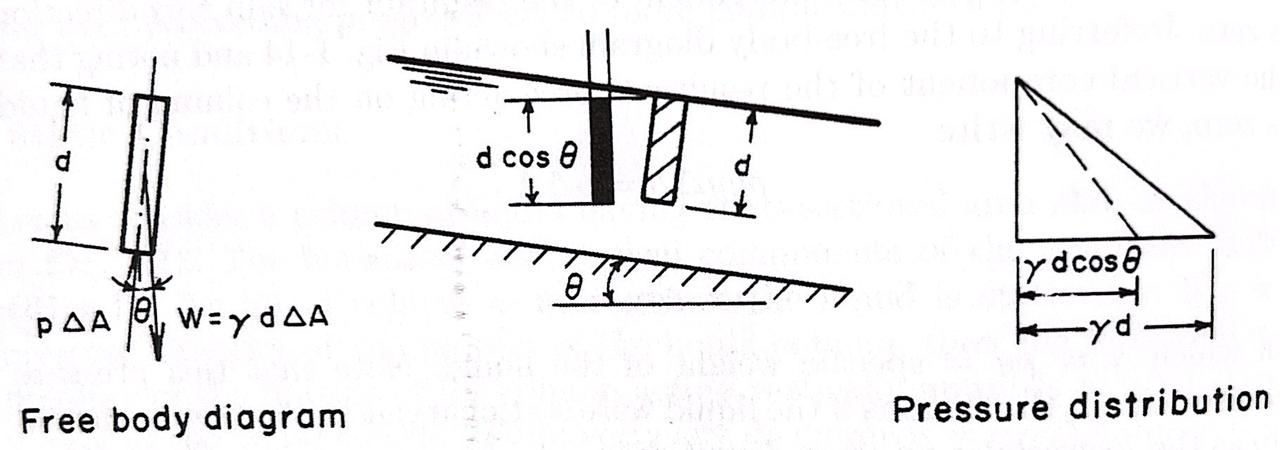
\includegraphics[width=8cm]{fig7.jpeg}
\caption{Curvas para calcular $y_n$ en canales canales circulares y trapezoidales para diferentes valores de la pendiente lateral $s$ (tomado de \cite{VChow}).}
\label{fig7}
\end{figure}

El c\'alculo de $y_n$ se puede realizar mediante la aplicaci\'on de m\'etodos num\'ericos para la soluci\'on de ecuaciones implicitas. En la tabla~\ref{fnor4} se presenta la geometr\'ia para las secciones transversales t\'ipicas de canales artificiales.

\begin{table}[h!]
\centering
\begin{tabular}{l c c c}
 \hline
 Tipo & Perimetro(P) & Area(A) & Variable \\ [0.5ex]
 \hline\hline
Rectangular & $b + 2y_n$ & $by_n$ & $y_n$ \\
Triangular & $y_n \left( \frac{1}{\sin \theta_1} + \frac{1}{\sin \theta_2} \right)$ & $ \frac{y_n^2}{2} \left( \frac{1}{\tan \theta_1} + \frac{1}{\tan \theta_2}\right)$ & $y_n$ \\
Trapezoidal & $y_n \left( \frac{1}{\sin \theta_1} + \frac{1}{\sin \theta_2} \right) + b$ & $ \frac{y_n}{2} \left[ y_n \left(\frac{1}{\tan \theta_1} + \frac{1}{\tan \theta_2}\right) +2b \right]$  & $y_n$ \\
Circular & $2r\theta$ & $r^2 \left( \theta -\frac{\sin 2\theta}{2} \right)$ & $\begin{aligned} y_n = r  &\text{\hspace{0.5cm} Si $\theta = 90$} \\ y_n = r(1-\cos \theta) &\text{\hspace{0.5cm} Si $0 < \theta < 90$} \\ y_n = r(1+\sin \theta) &\text{\hspace{0.5cm} Si $90 < \theta < 180$} \end{aligned}$ \\
\hline
\end{tabular}
\caption{Propiedades geom\'etricas para diferentes secciones transversales de un canal. La notaci\'on de las ecuaciones se puede observar en figura~\ref{fnor5}.}
\label{fnor4}
\end{table}

% LAM 
\begin{figure}[h]
\centering
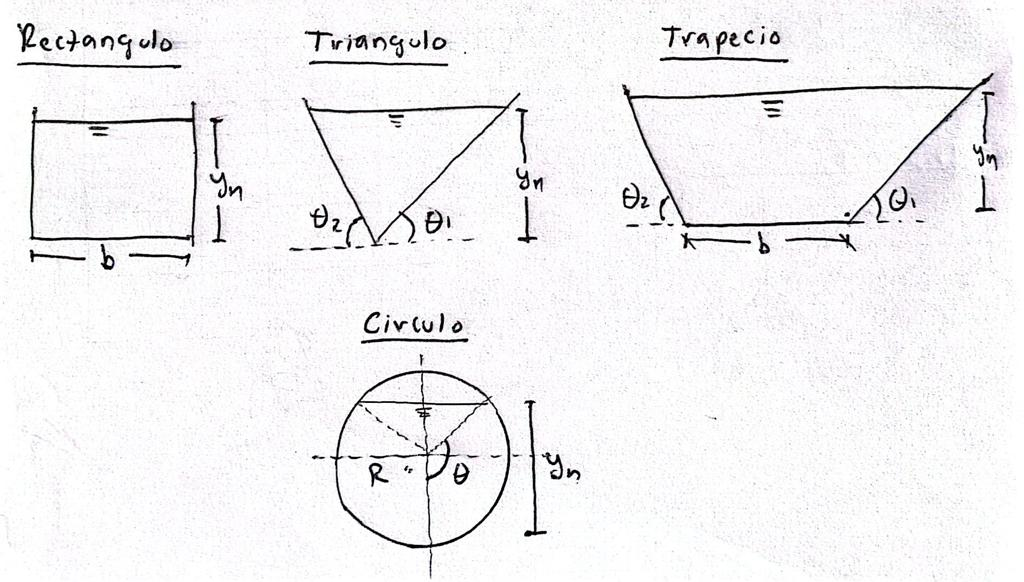
\includegraphics[width=8cm]{fnor5.jpeg}
\caption{Notaci\'on en canales artificiales usada en la tabla~\ref{fnor4}.}
\label{fnor5}
\end{figure}

Reemplazando $R = \frac{A}{P}$ en la ecuaci\'on~\ref{eq16} para cualquiera de las secciones de la tabla~\ref{fnor4}, se obtiene una ecuaci\'on implicita en $y_n$, con exepci\'on de la seccion circular en donde la funci\'on es implicita para $0^o < \theta < 180^o$.  La ecuaci\'on a resolver es:

\begin{equation}
\color{red}\boxed{\color{black}
\begin{split}
& f(y_n) = Q - A\frac{C_o }{n} R^{2/3} S_o^{1/2} = 0 \hspace{2cm} \text{Para todas las secciones exepto la circular}\\
& f(\theta) = Q - A\frac{C_o }{n} R^{2/3} S_o^{1/2} = 0 \hspace{2cm} \text{Para la secci\'on circular}\\
\end{split}
}
\label{fno8}
\end{equation}

Para resolver la ecuaci\'on~\ref{fno8}, se presenta a continuaci\'on un procedimiento con base en el \emph{m\'etodo de bisecci\'on}:
\begin{alg}{Calculo de $y_n$ por el m\'etodo de la bisecci\'on en canales artificiales}{alg1}
\begin{enumerate}
\item Leer la siguiente informacion:

\begin{enumerate}
\item Para la todas las secciones exepto la circular leer: $n$, $C_o$, $S_o$, $Q$, $b$, $\theta_1$ y $\theta_2$. Note que para la secci\'on rectangular $\theta_1 = \theta_2 = 90^o$, y para la secci\'on triangular $b=0$.
\item Para la secci\'on circular leer: $n$, $C_o$, $S_o$, $Q$, $R$ y $\theta$.
\end{enumerate}

\item Definir los l\'imites de iteraci\'on, $a$ y $b$, para el m\'etodo de bisecci\'on:
\begin{enumerate}
\item Para todas las secciones exepto la circular leer: $a = 0.01$ y $b=1000$ ($a \le y_n \le b$). Note que $y_n > 0$ y que $sign(f(a)) \neq sign(f(b)) $. Note que la funci\'on $sign$ extrae el signo de $f$.
\item Para la secci\'on circular leer: $a=0.01^o$ y $b=179.9^o$ ($a \le \theta \le b$). Note que $ 0^o < \theta < 180^o $, y que $sign(f(a)) \neq sign(f(b)) $. 
\end{enumerate}

\item \label{st5} Si $N <= Nmax=10000$ ir a ~\ref{st1}. Si $N > Nmax$ ir a ~\ref{st3}.  
\item \label{st1} Calcular $C = \frac{a+b}{2}$.
\item Calcular $f(c)$ usando la ecuaci\'on~\ref{fno8}. Si $|f(c)|< Error$ o $\frac{b-a}{2} < Error$ ir a ~\ref{st2}. Si no se cumple alguna de estas  condiciones ir a ~\ref{st4}.

\item \label{st4} Si $sign(f(c))$ = $sign(f(a))$, $a=c$, si no $b=c$. Incrementar $N=N+1$ e ir ~\ref{st5}. 

\item \label{st2} Imprimir:
\begin{enumerate}
\item para todas las secciones exepto la circular: $y_n = c$.
\item para la secci\'on circular: $\theta = c$. Usar las ecuaciones de la tabla~\ref{fnor4} para convertir $\theta$ en $y_n$.
\end{enumerate}

\item \label{st3} Ha fallado la iteraci\'on. Revisar datos de entrada y l\'imites iniciales de iteraci\'on.

\end{enumerate}
\end{alg}

% Ej 10.3 White 
\begin{eje}{}{eje1}
Un canal trapezoidal en asfalto ($n=0.016$) y con $S_o = 0.0015$, transporta agua con un caudal de 300 $ft^3 s^{-1}$. Si el ancho del canal es $b=6$ $ft$ y $\theta_1 = \theta_2 = 50^o$, calcular la profundidad normal ($y_n$).
\end{eje}

% seccion 10.2 White 
\begin{eje}{}{eje2}
Determinar para que relaciones de $y_n /D$ es posible transportar un caudal m\'aximo y obtener una velocidad m\'axima en un canal de secci\'on circular.
\end{eje}

\subsection{Canales naturales}
En la naturaleza, los canales por los cuales transcurre flujo poseen secciones irregulares como en el caso de rios y quebradas. Dicha secci\'on cambia en el tiempo debido a procesos de erosion y sedimentaci\'on en el fondo y en las orillas producto de cambios en la hidrodin\'amica del flujo. El c\'alculo de la profundidad normal se hace con base en la soluci\'on de la ecuaci\'on de Manning implicita para $y_n$ siguiendo un m\'etodo num\'erico. Si tenemos una secci\'on irregular de un canal como el mostrado en la figura~\ref{irre1}, conformada por una serie de $m$ puntos $p(x,y)$ con coordenadas espaciales $x$ y $y$, y cuyos coeficientes de Manning estan dados entre cada par de puntos $p_i$ y $p_{i+1}$ (segmento) para un total de $m-1$ coeficientes, el \'area mojada de la secci\'on para un valor de $y_n$ se puede calcular como:

% LAM 
\begin{figure}[h!]
\centering
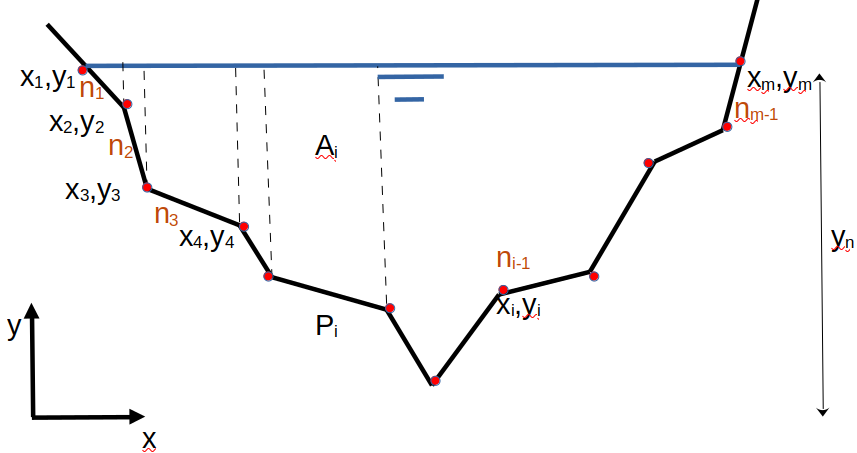
\includegraphics[width=8cm]{irre1.png}
\caption{Secci\'on transversal de un cauce irregular (e.g. rio).}
\label{irre1}
\end{figure}


\begin{equation}
A = \sum_{i=1}^{m-1} A_i = \sum_{i=1}^{m-1} \left[ (y_n - y_i )+(y_n - y_{i+1}) \right] \frac{x_{i+1}-x_i }{2}
\label{irr1}
\end{equation}

, perimetro se puede calcular como:

\begin{equation}
P = \sum_{i=1}^{m-1} P_i = \sum_{i=1}^{m-1} \sqrt{ (x_i - x_{i+1} )^2 + (y_i - y_{i+1})^2 }
\label{irr2}
\end{equation}

y el coeficiente de rugosidad de Manning como:

\begin{equation}
n = \left( \frac{\sum_{i=1}^{m-1} P_i n_i^{3/2}}{\sum_{i=1}^{m-1} P_i} \right)^{2/3}
\label{irr3}
\end{equation}

Note que la ecuaci\'on~\ref{irr1} c\'alcula el \'area mediante la sumatoria de las areas individuales (trapecios) $A_i$ formadas entre cada par de puntos $p_i$ y $p_{i+1}$, el perimetro en la ecuaci\'on~\ref{irr2} es la sumatoria de las distancias Euclidianas entre cada par de puntos $p_i$ y $p_{i+1}$ y el coeficiente de rugosidad de Manning  se obtiene unsando la ecuacion de Horton y Einstein, 1934. Note que $P_i$ en la ecuaci\'on~\ref{irr3} se obtine utilizando la ecuaci\'on~\ref{irr2}.

A continuaci\'on se muestra un procedimiento para el c\'alculo de $y_n$ en canales con secci\'on irregular basado en el m\'etodo de bisecci\'on:
\begin{alg}{Calculo de $y_n$ por el m\'etodo de la bisecci\'on en canales naturales}{alg2}
\begin{enumerate}
\item Leer la siguiente informaci\'on: $n$, $\alpha$, $S_o$, $Q$, $xs$, $ys$ y $ns$. Note que $xs$ y $ys$ son dos vectores con las coordenadas $x$ y $y$ respectivamente para un numero $m$ de puntos que conforman la seci\'on transversal. $ns$ es un vector de coeficientes de Manning para los $m-1$ segmentos que conforman la seccion.

\item Definir los l\'imites de iteraci\'on, $a$ y $b$, para el m\'etodo de bisecci\'on: $a = 0.01$ y $b=1000$ ($a \le y_n \le b$). Note que $y_n > 0$ y que $sign(f(a)) \neq sign(f(b)) $. Note que la funci\'on $sign$ extrae el signo de $f$.

\item \label{st5} Si $N <= Nmax=10000$ ir a ~\ref{st1}. Si $N > Nmax$ ir a ~\ref{st3}.  
\item \label{st1} Calcular $C = \frac{a+b}{2}$.
\item Con base en las coordenadas datas ($xs$ y $ys$), interpolar un nuevo conjunto de puntos para las profundidades normales $a$, $b$ y $c$.   
\item Calcular $f(a)$, $f(b)$ y $f(c)$ usando la ecuaci\'on ecuaci\'on~\ref{fno8} usando la nuevas secciones interpoladas para $a$, $b$ y $c$. Note que para evaluar la funci\'on es necesario, para cada nuevo conjunto de puntos, calcular el \'area (ecuaci\'on~\ref{irr1}), el perimetro (ecuaci\'on~\ref{irr2}) y la rugosidad de Manning (ecuaci\'on~\ref{irr3}.
\item Si $|f(c)|< Error$ o $\frac{b-a}{2} < Error$ ir a ~\ref{st2}. Si no se cumple alguna de estas  condiciones ir a ~\ref{st4}.

\item \label{st4} Si $sign(f(c))$ = $sign(f(a))$, $a=c$, si no $b=c$. Incrementar $N=N+1$ e ir ~\ref{st5}. 

\item \label{st2} Imprimir: $y_n = c$.
\item \label{st3} Ha fallado la iteraci\'on. Revisar datos de entrada y l\'imites iniciales de iteraci\'on.
\end{enumerate}
\end{alg}

%%%%%%%%
\section{Problemas de calculo en flujo uniforme} % From VChow 
El analisis de flujo uniforme se hace a trav\'es de una ecuacion de resistencia como la ecuaci\'on de Manning y la ecuacion de continuidad. Los problemas de flujo uniforme involucran las siguientes variables: caudal de flujo $Q$, coeficiente de rugosidad de Manning $n$, la profundidad de normal $y_n$, la velocidad de flujo $V$ y la pendiente del canal $S_o$. De acuerdo con esto, es posible encontrarse con alguno de los siguientes problemas:
\begin{enumerate}
\item \emph{Calculo del caudal $Q$}: En aplicaciones practicas se requiere para determinar la capacidad de transporte de un canal determinado, o para la construcci\'on de una curva de calibracion sintetica del canal.  
\item \emph{Calculo de la velocidad $V$}: Se requiere para el estudio de la erosion y sedimentaci\'on en canales. 
\item \emph{Calcular la profundidad normal $y_n$}: Calculo requerido para establecer el nivel de la lamina de agua en un canal (ver secci\'on~\ref{ynorm}).
\item \emph{Calculo de la rugosidad del canal $n$}: Se calcula el $n$ del canal y puede usarse para la soluci\'on de otros problemas en canales en condiciones similares. 
\item \emph{Calculo de la pendiente del canal $S_o$}: Se calcula para determinar la pendiente requerida de un canal determinado bajo ciertas condiciones de flujo y rugosidad. 
\end{enumerate}
Analisando lo anterior, la soluci\'on de cualquiera de los anteriores problemas, exepto el del calculo de $y_n$, se hace usando la ecuacion de Manning y la ecuacion de continuidad de manera explicita por lo que su calculo es relativamente simple.


%%%%%%%%
\section{Diseño de canales} % From Chau
El diseño de canales involucra la selecci\'on del trazado, forma de la secci\'on, pendiente del fondo, velocidad permitida y recubrimiento. Cabe aclarar que canales recubiertos ofrecen menor fricci\'on por lo que el tamano de la secci\'on para un caudal determinado es menor que para un canal sin recubrimiento. El diseño de canales se hace asumiendo flujo uniforme y el calculo se hace por prueba y error de tal manera que de acuerdo con los requierimientos del diseño y los parametros escogidos el canal se operativamente viable. Esto quiere decir el factor decisivo es el economico, es decir, se escoge el diseño mas barato entre una combinacion de alternativas todas operativamente posibles. Este analisis de costos debe incluir los costos operativos y de mantenimiento. En muchos casos se asume flujo gradualmente variado de tal manera que el tamano del canal sea determinado de forma optima. El diseño de canales se puede dividir en dos categorias: canales no erosionables (recubrimiento rigido) y canales erosionables (no recubiertos).

\subsection{Canales no erosinables}
En el diseño de canales no erosinables, se escoge el tipo de secci\'on, el material de recubrimiento y el tamaño de tal manera que el canal sea capaz de transportar el caudal de diseño con un borde libre ($F_b$) que se define como la diferencia entre la superficie del agua (de acuerdo con $y_n$) y la parte superior de las bancas del canal en unidades de longitud. Ese borde libre tiene en cuenta la incertidumbre de los calculos y de los parametros escogidos, asi como perturbaciones del flujo (e.g. olas). De acuerdo con U.S. Bureau of Reclamation, $F_b = \sqrt{k y}$, donde $y$ es la profundidad del agua en metros y $k$ es un factor igual a 0.8 para caudales cercanos a 0.5 m$^3$ s$^{-1}$, e igual 1.4 para caudales mayores 85  m$^3$ s$^{-1}$. 

La alineaci\'on del canal debe ser tal manera que sea lo mas corto posible permitiendo el facil acesso para el mantenimiento asi como otras consideraciones constructivas. La pendiente es determinada por la topografia y junto con la forma y el tamaño de la secci\'on deben garantizar el transporte del caudal de diseno y minimizar los costos de su construcci\'on. La velocidad debe garantizar que no haya erosion del material de revestimiento asi como la no sedimentacion de material. Las velocidades minimas en un canal varian entre 0.6 y 0.9 m/s y velociades por debajo de 12 m/s con flujo bajo en sedimentos son apropiadas en canales de concreto. Es comun entonces encontrar que canales rectangulares son comunes para el transporte de caudales menores (e.g. cunetas de vias) mientras que canales trapezoidales son construidos para transportar mayores caudales (e.g. aguas lluvias en ciudades). Los canales de secc\'ion circular son comunes en el paso de vias y a traves de sistemas rocosos. 


\begin{alg}{Diseño de canales no erosionables}{alg1}
\begin{enumerate}
\item Lea el caudal $Q$ de diseño y $C_o$.
\item \label{st2} Seleccione el material de revestimiento y con esto el $n$ de Manning. Con base en la topografia y aspectos constructivos, selecciones la pendiente del canal $S_o$.
\item \label{st3} Para unos valores escogidos de la geometria del canal como la base $b$ y la pendiente lateral $s$, resolver la ecuaci\'on de Manning (ecuaci\'on~\ref{eq16}) para encontrar $y_n$. Este proceso es iterativo teniendo en cuenta que se debe encotrar una relaci\'on $b/ y_n$ que garantize la mejor secci\'on hidraulica (ver secci\'on~\ref{secop}).
\item Con el fin de evitar procesos de sedimentaci\'on en el canal, revisar que $V > V_{min}$. Si esto es falso, ir a los pasos~\ref{st2} y ~\ref{st3} y revisar estos parametros. Si es verdad, ir al paso~\ref{st5}. 
\item \label{st5} Agregar un borde libre $F_b$ al canal.
\end{enumerate}
\end{alg}

% Ej 9.1 Chau 
\begin{eje}{}{eje1}
Diseñar un canal trapezoidal para transportar un caudal de 10 m$^3$ s$^{-1}$. El canal canal sera escavado en roca ($n=$ 0.030) y la pendiende del terreno es 4000:1. La pendiente lateral $s$ es 1:4. 
\end{eje}


\subsection{Secci\'on \'optima de un canal}\label{secop}
El dise\~no de canales en ingenier\'ia requiere determinar la secci\'on \'optima (aquella que garantice la menor resistencia al flujo) en un canal para unas condiciones dadas. Usando la ecuaci\'on de Manning (ecuaci\'on~\ref{fno7}) es posible maximizar el radio hidr\'aulico ($R_h$) para un \'area ($A$) y un caudal ($Q$) dado. Teniendo en cuenta que $R_h = A/P$, para maximizar $R_h$ debemos minimizar el per\'imetro ($P$). 

Considerando el canal trapezoidal de la figura~\ref{fnor6}, el area y el perimetro se pueden calcular como:
% Fig 10.7 White 
\begin{figure}[h!]
\centering
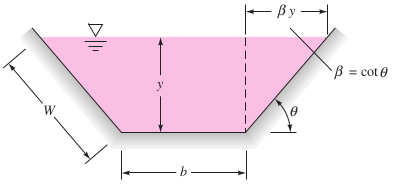
\includegraphics[width=8cm]{fnor6.png}
\caption{Geometria de un canal trapezoidal (tomado de \cite{white1990fluid}).}
\label{fnor6}
\end{figure}

\begin{equation}
A = b y + \beta y^2
\label{fni1}
\end{equation}

\begin{equation}
P = b + 2W = b + 2y \left( 1+\beta^2 \right)^{1/2}
\label{fni2}
\end{equation}
donde $\beta = \cot \theta$ y $y=y_n$. Note que $W = \sqrt{y^2 \beta^2 + y^2}= y \left( \beta^2 +1 \right)^{1/2}$. Asumiendo que $b$ es un dato dado, se despeja de la ecuaci\'on~\ref{fni1}:

\begin{equation}
b = \frac{A}{y}- y\beta
\label{fni3}
\end{equation}

y de la ecuaci\'on~\ref{fni2}:

\begin{equation}
b = P -2y \left( 1+\beta^2 \right)^{1/2}
\label{fni4}
\end{equation}

igualando las ecuaciones~\ref{fni3} y ~\ref{fni4} y despejando para $P$, se tiene:

\begin{equation}
P = \frac{A}{y} - y\beta + 2y\left( 1+\beta^2 \right)^{1/2}
\label{fni5}
\end{equation}

Para minimizar $P$, se obtiene $dP/dy$ de la ecuaci\'on~\ref{fni5} tomando como constantes $A$ y $\beta$:

\begin{equation}
\frac{dP}{dy} = -\frac{A}{y^2} - \beta + 2\left( 1+\beta^2 \right)^{1/2}
\label{fni6}
\end{equation}

igualando $dP/dy=0$ y despejando $y$ se optiene el valor de $y$ que minimiza $P$:

\begin{equation}
y = \left[ \frac{A}{2\left( 1+\beta^2 \right)^{1/2} - \beta} \right]^{1/2}
\label{fni7}
\end{equation}

Despejando $A$ de la ecuaci\'on~\ref{fni7} y reemplazando en la ecuaci\'on~\ref{fni5} para $P$, la geometr\'ia optima de un canal trapezoidal para un angulo $\theta$ dado es:

\begin{equation}
\color{red}\boxed{\color{black} A = y^2 \left[ 2\left( 1 + \beta^2 \right)^{1/2} - \beta \right] \hspace{1cm} P=4y\left( 1 + \beta^2 \right)^{1/2} -2\beta y \hspace{1cm} R_h = \frac{y}{2}}
\label{fni8}
\end{equation}

La ecuaci\'on~\ref{fni8} indica que para un angulo $\theta$ dado, la secci\'on transversal mas eficiente de un canal en flujo uniforme ocurre cuando el radio hidr\'aulico es igual a la mitade la profundidad normal. Igualando las ecuaci\'ones~\ref{fni2} y ~\ref{fni8} para $P$, se tiene una expresi\'on para la base inferior del canal $b$:

\begin{equation}
b = 2y\left(\sqrt{1+\beta^2} - \beta \right)
\label{fni8a}
\end{equation}
 
y la base superior $b_s$
\begin{equation}
b_s =b+2\beta y = 2y\left(\sqrt{1+\beta^2} \right)
\label{fni8b}
\end{equation}

Teniendo en cuenta que cuando $\theta = 90^o$ $\beta = 0$ por lo que tenemos un canal rectangular, reemplazando esto en las ecuaciones~\ref{fni8} se tiene la secci\'on m\'as eficiente para un canal rectangular:
    
\begin{equation}
\color{red}\boxed{\color{black} A = 2y^2 \hspace{1cm} P=4y  \hspace{1cm} R_h = \frac{y}{2} \hspace{1cm} b = 2y }
\label{fni9}
\end{equation}

Para encontrar la profundidad correcta, es necesario solucionar las ecuaciones anteriores en conjunto con la ecuaci\'on~\ref{fno7} para un caudal dado. 

Es posible encontrar el mejor angulo $\theta$ del canal trapezoidal para un \'area y una profundidad dada. Evaluando $dP/d\beta$ para $A$ y $y$ constante se tiene:

\begin{equation}
\frac{dP}{d\beta} = -y +2\beta y\left( 1 + \beta^2 \right)^{-1/2} 
\label{fni10}
\end{equation}

igualando la ecuaci\'on~\ref{fni10} a cero se tiene:

\begin{equation}
2\beta = \left( 1 + \beta^2 \right)^{1/2} \hspace{1cm} \beta=\cot \theta = \frac{1}{\sqrt{3}} \hspace{1cm} \theta=60^o
\label{fni10}
\end{equation}

Esto indica que para una profundidad dada, el angulo $\theta$ \'optimo es $60^o$, o que la secci\'on \'optima (la que maximiza el flujo) es la mitad de un hex\'agono. 

Si se circunscribe una secci\'on circular de radio $R$ en la secci\'on trapezoidal donde $\theta=60^o$, se tiene que $R=\frac{1}{2}b_s \sin \theta$. Reemplazando $b_s$ en esta ecuaci\'on y sabiendo que $\beta=\frac{1}{\sqrt{3}}$, se tiene que $R=y$. Esto demuestra que una secci\'on circular tiene su m\'axima eficiencia cuando $y=R$ (semicirculo). 

Para una secci\'on triangular ($b=0$ en la figura~\ref{fnor6}), el \'area y el per\'imetro son:
\begin{equation}
A = \beta y^2
\label{fni11}
\end{equation}

\begin{equation}
P = 2W =  2y \left( 1+\beta^2 \right)^{1/2}
\label{fni12}
\end{equation}

Despejando $y$ de la ecuaci\'on~\ref{fni11} se tiene que $y = \left( \frac{A}{\beta} \right)^{1/2}$. Reemplazando en la ecuaci\'on~\ref{fni12}, el per\'imetro es:

\begin{equation}
P = 2W =  2\left(\frac{A}{\beta}\right)^{1/2} \left( 1+\beta^2 \right)^{1/2}
\label{fni13}
\end{equation}

derivando $P$ con respecto a $\beta$ en la ecuaci\'on~\ref{fni13}, se tiene:

\begin{equation}
\frac{dP}{d\beta} =2A^{1/2}\left[ \beta \left( 1+\beta^2 \right)^{-1/2} \beta^{-1/2} - \frac{1}{2} \frac{\left( 1+\beta^2 \right)^{1/2}}{\beta^{3/2}} \right]
\label{fni14}
\end{equation}

Haciendo $dP/d\beta = 0$, se tiene:

\begin{equation}
\frac{\beta^{1/2}}{\left( 1+\beta^2 \right)^{1/2}} = \frac{\left( 1+\beta^2 \right)^{1/2}}{2 \beta^{3/2}}
\label{fni15}
\end{equation}

Solucionando la ecuaci\'on~\ref{fni15}, se tiene que $\beta=1$. Esto quiere decir que una secci\'on triangular con $\theta=45^o$ es la mas eficiente.

% Ej 10.4 White 
\begin{eje}{}{eje1}
Para un canal rectangular en ladrillo ($n=0.015$) dise\~nado para transportar 5 $m^3 /s$ y con una pendiente de $S_o = 0.001$, determinar las mejores dimensiones para $y$ y $b$. Realizar los mismos c\'alculos si la secci\'on transversal del canal es la mitad de un hex\'agono y si es un semicirculo. Comparar los resultados.  
\end{eje}


\subsection{Canales erosinables}
Para canales excavados en terrenos blandos sin ningun tipo de revestimiento, es posible que se presente erorosion de la secci\'on si no se escoge un tamaño y una pendiente adeacuados. Existen dos metodos para el analisis de este tipo de canales que son tratados a continuacion.

\subsubsection{Metodo de la velocidad permisible}
El tamaño de la secci\'on del canal se escoge de tal manera que $V$, bajo el supuesto de flujo uniforme, sea menor a una \emph{velocidad permisible}. Esta velocidad permisible es aquella para la cual no se presenta erosion en la secci\'on del canal. Esta velocidad depende principalmente del tipo de suelo y del tamaño de las particulas. Sin embargo tambien depende de la profundidad de agua y de la alineacion del canal. Esto debido a que para la misma velocidad media del flujo, la velocidad el flujo en el fondo en mayor cuando la profundidad es baja que cuando es alta. De la misma manera, canales curvos presentan corrientes secundarias que que aceleran el flujo hacia la parte externa de la curva causando erorsionen las orillas. 

La secci\'on trapezoidal es la mas usada y las pendiente laterale $s$ deben ser escogida de tal manera que garantice la estabilidad del material en las orillas. La tabla~\ref{ta5} presenta valores recomendados de $s$ para diferentes tipos de material. De manera similar, la tabla~\ref{ta6} presenta valores de velocidades permisibles para diferentes materiales en canales rectosy profundidad de agua de 1 m. En el caso de canales con algo de sinuosoidad, la velocidad permisible se debe reducir en 5\%, para canales con sinuosoidad media, la velocidad se debe reducir en 13\% y para canales con alta sinuosouidad, la velocidad se debe reducir en 22\%. Para canales muy anchos y con profundidades diferentes a un 1 m, la velocidad permisible se debe multiplicar por un factor de correcci\'on $k=y^{1/6}$, donde $y$ es la profundidad del flujo. 

\begin{table}[h!]
\centering
\begin{tabular}{l c}
 \hline
  Material & $s$ \\ [0.5ex]
 \hline\hline
 Roca & Casi vertical \\
 Arcilla resistente & 1:0.5 hasta 1:1 \\
 Suelo firme & 1:1 \\
 Suelo arenoso & 2:1 \\
 Suelo con arenas, arcilla y limos & 3:1 \\
\hline
\end{tabular}
\caption{Pendiente lateral en canales trapezoidales (tomado de \cite{Chau}).}
\label{ta5}
\end{table}

\begin{table}[h!]
\centering
\begin{tabular}{l c}
 \hline
  Material & $V$ (m/s) \\ [0.5ex]
 \hline\hline
 Arena fina & 0.6 \\
 Arena gruesa & 1.2 \\
\emph{Suelo} & \\
- limo arenoso & 0.6 \\
- limo arcilloso & 1.1 \\
- arcilloso & 1.8 \\
\emph{Suelo con pasto Bermuda} & \\
- limo arenoso & 1.8 \\
- limo arcilloso & 2.4 \\
\emph{Suelo con pasto Kentucky} & \\
- limo arenoso & 1.5 \\
- limo arcilloso & 2.1 \\
\emph{Roca blanda} & \\
- arenisca blanda & 2.4 \\
- lutita blanda & 1.1 \\
Roca dura  & 6.1 \\
\hline
\end{tabular}
\caption{Velocidades permisibles (tomado de \cite{Chau}).}
\label{ta6}
\end{table}

\begin{alg}{Diseño de canales erosionables: m\'etodo de la velocidad permisible}{alg1}
\begin{enumerate}
\item Leer el caudal $Q$ de diseño, la pendiente del canal $S_o$ y $C_o$.
\item \label{st2} De acuerdo con el material excavado, seleccione el $n$ de Manning, el $s$ de acuerdo con la tabla~\ref{ta5}, y la velocidad permisible $V$ de la table~\ref{ta6}.
\item De la ecuaci\'on de Manning (ecuaci\'on~\ref{eq16}), calcular $R$.
\item De la ecuaci\'on de continuidad, $Q=AV$, calcular $A$.
\item Calcular el perimetro mojado $P$, a partir de $P=A/R$.
\item De las ecuaciones para $P$ y $A$, estimar el ancho del canal $b$ y la profundidad normal $y_n$.
\item \label{st5} Agregar un borde libre $F_b$ al canal.
\end{enumerate}
\end{alg}

% Ej 9.2 Chau 
\begin{eje}{}{eje1}
Diseñar un canal para transportar un caudal de 6.91 m$^3$ s$^{-1}$. El canal sera excavado en arcilla resistente con una pendiente del terreno $S_o = 0.00318$.
\end{eje}

\subsubsection{M\'etodo de la fuerza tractiva}
La erosion de las part\'iculas del material de la secci\'on de un canal se puede comprender mejor a trav\'es del an\'alisis de la \emph{fuerza tractiva}. El an\'alsis de fuerzas indica que una part\'icula de material permanecer\'a estable si las fuerzas de cohesi\'on son mayores que las \emph{fuerzas de arrastre} debido a los esfuerzos cortantes ejercidos por el flujo sobre las paredes y el fondo del canal. Para flujo uniforme en una canal recto, la fuerza tractiva es igual a la componente del peso del fluido en la direcci\'on del flujo. 

Si se considera un canal recto de longitud $L$, con un area mojada $A$ y con pendiente $S_o$, el peso del volumen del fluido para $L$ es $\gamma A L$. De acuerdo con esto, la componente de dicho peso en la direccion del flujo es $\gamma A L S_o$ (note que para $S_o$ pequeñas, $\sin \theta \approx \tan \theta \approx S_o$). La fuerza tractiva por unidad de area o el esfuerzo cortante sobre el area mojada del tramo de canal $PL$, se define como $\tau_o = \frac{\gamma A L S_o}{PL} = \gamma R S_o$, donde $R$ es el radio hidr\'aulico. Para canales muy anchos, $R \simeq y$ por lo tanto $\tau_o = \gamma y S_o$. La distribuci\'on de esfuerzos cortantes o de fuerza tractiva por unidad de area sobre la seccion del canal no es uniforme. Sin embargo se ha encontrado que para canales trapezoidales anchos, $\tau_o = \gamma y S_o$ en el fondo y en las paredes $\tau_o = 0.76 \gamma y S_o$. 

El esfuerzo cortante necesario para iniciar el movimiento de una part\'icula se denomina \emph{esfuerzo cortante cr\'itico} $\tau_c$ y depende del tamano del material y de la cohesion de las part\'iculas. Note que este esfuerzo es mayor para part\'iculas sobre el fondo que para part\'iculas sobre las paredes del canal, ya que el movimiento de esas ultimas esta influeciada por la gravedad. Considere una part\'icula de material sobre la pared de un canal cuyo angulo de inclinacion de la pared del canal es $\theta$, $a$ es el area efectiva de la part\'icula, $W_s$ es el peso sumergido de la part\'icula, $\phi$ es el angulo de reposo del materia  y $\tau_s$ es el esfuerzo cortante sobre las paredes del canal  (ver figura~\ref{fnor7}). 

% Fig 9.2 Chau 
\begin{figure}[h!]
\centering
%\includegraphics[width=8cm]{fnor7.png}
\caption{Fuerzas actuantes sobre una part\'icula en una pared de un canal (tomado de \cite{Chau}).}
\label{fnor7}
\end{figure}

Existen dos fuerzas que tienden a desequilibrar la part\'icula: 1) la fuerza tractiva que se calcula como $\tau_s a$, y la componente del peso de la part\'icula a lo largo de la pared del canal $W_s \sin \theta$. La resultante de estas dos fuerzas es:

$$
R=\sqrt{W_s^2 \sin^2 \theta + a^2 \tau_s^2}   
$$

La fuerza normal a la pared del canal se calcula como $W_s \cos \theta \tan \phi$ y evita el movimiento de la part\'icula. La part\'icula est\'a en equilibrio si las fuerzas que propician el movimiento son iguales a las que se oponen a este, por lo que:

$$
W_s \cos \theta \tan \phi =\sqrt{W_s^2 \sin^2 \theta + a^2 \tau_s^2}   
$$

Despejando de esta ecuaci\'on $\tau_s$, se tiene:

\begin{equation}
\tau_s = \frac{W_s}{a}\cos \theta \tan \phi \sqrt{1-\frac{\tan^2 \theta}{\tan^2 \phi}}
\label{fni16}
\end{equation}

La fuerza que impide el movimiento sobre una superficie nivelada es $W_s \tan \phi = a \tau_l$, donde $\tau_l$ es el esfuerzo cortante que impide el movimiento de la particula sobre una superficie nivelada. Por lo tanto:

$$
\tau_l = \frac{W_s}{a} \tan \phi
$$

Reemplanzado en la ecuaci\'on~\ref{fni16}, se tiene:
\begin{equation}
K = \frac{\tau_s}{\tau_l} = \cos \theta \sqrt{1-\frac{\tan^2 \theta}{\tan^2 \phi}}
\label{fni17}
\end{equation}

donde $K$ se denomina el factor de reducci\'on del esfuerzo critico sobre las paredes del canal.

Los efectos debido al angulo de reposo del material se consideran para material grueso sin cohesi\'on. Para material fino cohesivo y no cohesivo, la componente del peso a lo largo de la pared es muy pequeña con respecto a las fuerzas cohesivas por lo cual se pueden despreciar. La figura~\ref{fnor8} muestra el angulo de reposo para material no cohesivo cuyo diametro, para mas del 25\% del peso total del material, es $>5$ mm. Los esfuerzos criticos para material no cohesivo se muestran en la figura~\ref{fnor9} y para material cohesivo en la figura~\ref{fnor10} para canales rectos. Estos valores de $\tau_c$ deben reducirse en 10\% para canales algo sinuosos, en 25\% para canales moderadamente sinuosos y en 40\% para canales muy sinuosos. 

% Fig 9.3 Chau 
\begin{figure}[h!]
\centering
%\includegraphics[width=8cm]{fnor8.png}
\caption{Angulo de reposo ($\phi$) para material no cohesivo  para particulas de diametro $> 5$ mm (tomado de \cite{Chau}).}
\label{fnor8}
\end{figure}

% Fig 9.4 Chau 
\begin{figure}[h!]
\centering
%\includegraphics[width=8cm]{fnor9.png}
\caption{Esfuerzo cortante critico ($\tau_c$) para material no cohesivo (tomado de \cite{Chau}).}
\label{fnor9}
\end{figure}

% Fig 9.5 Chau 
\begin{figure}[h!]
\centering
%\includegraphics[width=8cm]{fnor10.png}
\caption{Esfuerzo cortante critico ($\tau_c$) para material cohesivo (tomado de \cite{Chau}).}
\label{fnor10}
\end{figure}

El diseño de canales por el m\'etodo de la fuerza tractiva involucra la escogencia de una secci\'on transversal de tal manera que la fuerza tractiva por unidad de \'area ($\tau_s$) actuante sobre las paredes del canal sea igual al esfuerzo critico ($\tau_c$) que resistiria el material del canal. Al final de la escogencia de la secci\'on, se debe cumplir que el esfuerzo cortante sobre el fondo del canal sea menor que $\tau_c$.

\begin{alg}{Diseño de canales erosionables: m\'etodo de la fuerza tractiva}{alg1}
\begin{enumerate}
\item Leer el caudal $Q$ de diseño, la pendiente del canal $S_o$ y $C_o$.
\item \label{st2} De acuerdo con el material excavado, seleccione el $n$ de Manning, el $s$ de acuerdo con la tabla~\ref{ta5}, el angulo de reposo $\phi$ del material a partir de la figura~\ref{fnor8} y el esfuerzo critico $\tau_c$ de la figura~\ref{fnor9}, si el material es no cohesivo, o de la figura~\ref{fnor10} si el material es cohesivo. Ajustar $\tau_c$ dependiendo de la sinusoidad del canal. 
\item Para material no cohesivo, calcular el factor de reducci\'on $K$ a partir de la ecuaci\'on~\ref{fni17}. Calcular el esfuerzo cortante de las paredes $\tau_s = K \tau_c$.
\item Igualar $\tau_s$, calculado en paso anterior, a $0.76\gamma y S_o$, de donde se determina $y=\frac{\tau_s}{0.76 \gamma S_o}$. 
\item De la ecuaci\'on de Manning (ecuaci\'on~\ref{eq16}), calcular $b$.
\item Revisa que el esfuerzo cortante en el fondo, $\tau = \gamma y S_o$, es menor que el $\tau_c$ determinado en el paso~\ref{st2}. Si se cumple ir a el paso~\ref{st5}, si no volver al paso~\ref{st2}. 
\item \label{st5} Agregar un borde libre $F_b$ al canal.
\end{enumerate}
\end{alg}

% Ej 9.3 Chau 
\begin{eje}{}{eje1}
Diseñar un canal trapezoidal recto para transportar un caudal de 10 m$^3$ s$^{-1}$. El canal sera excavado en grava fina de diametro 8 mm  con una pendiente del terreno $S_o = 0.00318$. Asumir que las particulas de grava son casi redondas y la concentraci\'on de sedimentos en suspensi\'on en el flujo es baja. 
\end{eje}



% REFERENCES
\bibliographystyle{plain} % We choose the "plain" reference style
\bibliography{refs} % Entries are in the refs.bib file

\end{document}
